%!TEX root = ../thesis.tex
%*******************************************************************************
%****************************** Second Chapter *********************************
%*******************************************************************************

\chapter{Background}
% \ifpdf
    \graphicspath{{Chapter2/Figs/Raster/}{Chapter2/Figs/PDF/}{Chapter2/Figs/}}
% \else
%     \graphicspath{{Chapter2/Figs/Vector/}{Chapter2/Figs/}}
% \fi

\section{Review of Relevant Education Research}

Identifying issues in traditional higher education today that a blockchain-based system can better 
tackle is one of the objectives of this project. This informs the scope of the 
project and the design of the deliverables.

There is an abundant amount of pedagogy and learning method research, which focuses on the 
instruments and mode of delivery. These include methods such as "scaffolding", "constructivism", 
"problem-based learning", and "active learning" \citep{ali2005effective}. However, this 
research area is considered out of the scope of discussion for this project, which does not 
aim to provide new insight into ICT-enhanced pedagogies, nor will it be designed around any 
preferred pedagogies. This project is interested in representing components of e-learning, 
such as delivery, assessment, and record keeping in a more generic, general purposed manner.

\subsection{Assessments and Transparency}

Assessment is arguably the most important process in the business of education as it "drives what 
is learnt and taught" and "convert learning into credentials". \citep[p.160]{campbell2010digital}

\citet{brown1999assessment} summarised examples of popular sentiments learners held about both 
continuous assessments and traditional exams, such as:

\begin{enumerate}
    \setlength\itemsep{0em}
    \item Assessment tasks do not increase students' want to learn, only their need to learn, promoting unhappiness;
    \item Invalid and unreliable marking due to speed or fatigue of assessors, plagiarism and unwanted collaborations, etc.;
    \item Sub-optimal levels of feedback after many types of assessments;
    \item Students feel forced into surface learning.\\
    \citep[p.62-65]{brown1999assessment}
\end{enumerate}

The importance of assessments, coupled with popular unhappiness and mistrust amongst learners towards 
them, grows the tension between the teacher (or educational provider) and the learners.

\citet{suhre2013determinants} looked into motivation on study progress in a higher education setting by collecting data 
from 168 first-year university students for six months. The study found three main factors that motivates academic 
progress: intrinsic abilities, personal motivations such as a need to achieve or fear of failure, and transparency in 
exams and assessments.

Transparency here refers to both the clarity of assessment goals and the procedures for assessing these goals. 
It should be clear to learners what knowledge is required for a sufficient level of mastery. \citep{suhre2013determinants}
The difference this makes was significant:

\begin{itemize}
    \setlength\itemsep{0em}    
  \item Students' perceptions of degree programme organization and transparency of exams are 
  significantly correlated with academic performance;
  \item Academic pressure is substantially influenced by the perceived transparency of assessments.
\end{itemize}

An improvement in the transparency of goals, procedures, knowledge required of assessments and an increase 
in feedback can directly tackle some of the negative sentiments listed above from \citet{brown1999assessment}, 
such as 1, 2 and 3.

\subsection{Personalisation in Education}

Personalisation is regarded as the solution to traditional bureaucratic state education that is irresponsive, 
inflexible, over-regulated, with the ‘one size fits all’ approach. The case for personalisation assumes that prior state 
provision was, if not actually totalitarian, certainly machine-like, crude, churning out standardised goods, insensitive to diversity. \citep{bragg2014review}

Current research into personalisation (or customisation) of education is broad and covers both the personalisation 
of pedagogy and curriculum. Notably, research points to a growing appreciation of the need to support and 
encourage learner control over the whole/entire learning process \citep{dron2007designing}.

\citet{green2005futurelab} summarised four key areas pivotal to enabling personalised learning through digital 
technologies. The pedagogy should:

\begin{itemize}
    \setlength\itemsep{0em}    
    \item ensure that learners are capable of making informed educational decisions;
    \item diversify and recognise different forms of skills and knowledge;
    \item create diverse learning environments; and
    \item include learner focused forms of feedback and assessment.
\end{itemize}

The design of a learning platform that aims at supporting personalisation must therefore focus on facilitating these 
four actions.



[TODO: Cover personalisation broadly and in terms of curriculum (which modules to take, 
customised passing thresholds) which can be negotiated on the blockchain.
To be added if there is time for the project to cover this area.]

% https://www.researchgate.net/publication/262901454_Education_%27consumerism%27_and_%27personalisation%27





(p.7)

http://onlinelibrary.wiley.com/doi/10.1111/j.1467-8527.2008.00411.x/full







\section{Literature Review in e-Learning}

E-learning has been growing as an industry and research area, and various standards have been devised. 
A review of these frameworks could provide valuable insights.

\subsection{e-Learning Systems}

\begin{figure}[!ht] 
    \centering    
    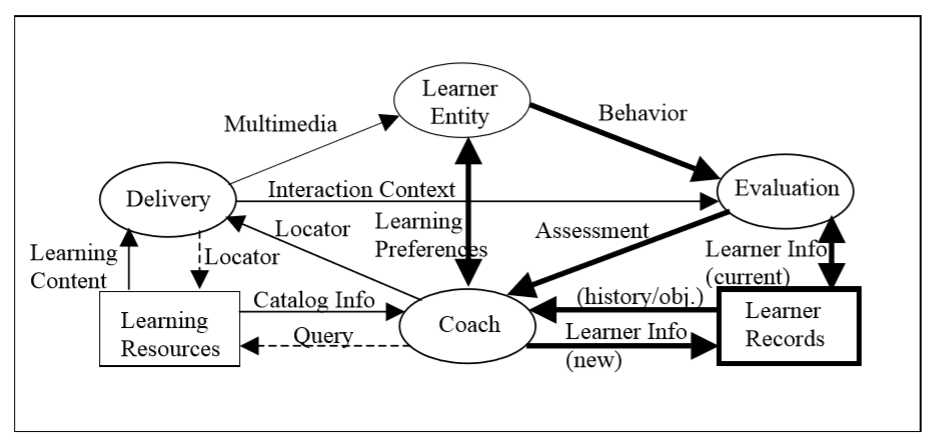
\includegraphics[width=1.0\textwidth]{LTSA}
    \caption[Learning Technology Systems Architecture]
        {Learning Technology Systems Architecture, IEEE P1484.1/D9 \citep{farance1999learning}}
    \label{fig:LTSA}
\end{figure}

IEEE P1484.1/D9: the Learning Technology Systems Architecture (LTSA) provides a valuable way of organising 
the scope and discussion in this project. It identified four main components: learner entity, coach, 
delivery and evaluation; and two main resources: learning resources and learner records (See figure \ref{fig:LTSA}).

Identifying the properties of a blockchain-based system that could improve these components is 
critical to this project. For example, the distributed, immutable storage of learner records could 
provide extra security.

\subsection{e-Learning Research Framework}

\citet{garrison2011learning} provided a framework for research and practice called the "Community 
of Inquiry (CoI)" framework, which included three main categories:

\begin{enumerate}
    \setlength\itemsep{0em}    
    \item Enhancing the social presence, such as collaborative learning
    \item Enhancing the cognitive presence, such as practical inquiry and critical thinking
    \item Enhancing the teaching presence, especially with asynchronous e-Learning (eg. pre-recorded lectures)
\end{enumerate}

A blockchain back-end could potentially provide experiential improvements in the above three categories as well. 
For example, smart contracts could enhance the social and teaching presence by facilitating teacher-learner, or 
learner-learner negotiations.

% \subsection{Self-Regulation and Motivation}

% There are several dimensions of self-regulation that will help a learner stay on an 
% e-Learning course or curriculum:

% \begin{table}[!ht] 
%     \caption{Self-Regulation and Motivation Strategies, adapted from \citep[p.189]{o2013web}}
%     \centering
%     \label{table:Self-regulation Dimensions}
%     \begin{tabular}{l c }
%         \toprule
%         Self-regulation Dimensions & Examples of Motivation Strategies \\ 
%         \midrule
%         Motives & Setting challenging but achievable goals \\ \hline
%         Methods of Learning & Summarisation, outline-formatted notes, \\
%         & interrogation and rehearsal, etc\\ \hline
%         Time Management & Prioritizing tasks, dealing with procrastination\\ \hline
%         Physical Environment & An environment conducive to learning\\ \hline
%         Social environment & Help seeking: knowing when help is needed,\\
%         & identifying sources of help, framing help request,\\
%         & evaluating help received\\ \hline
%         Performance & Observing and reflecting upon performance\\
%         & with short-term and long-term goals\\
%         \bottomrule
%     \end{tabular}
% \end{table}

% An e-learning programme should equip a learner with these self-regulation skills,
% and the e-learning system should provide tools that facilitate and enable the 
% motivation strategies.

\subsection{Security and Privacy}

The security of e-learning systems have also been a concern. For example, \citet{el2003privacy} noted that “while many 
advances have been made in the mechanics of providing online instruction, the needs for privacy and security have to-date 
been largely ignored. At best they have been accommodated in an ad-hoc, patchwork fashion.”

The consequences of cybersecurity breaches have also become more and more expensive. For example, when the General Data 
Protection Regulation (GDPR) comes into effect across Europe in May 2018, the maximum fine for poor practices and data 
breaches will be £17 million or 4\% of global turnover \citep{ico2017gdpr}.

The scale and severity of historic breaches of of internet services has been worrying. Most notably in the e-learning 
industry, the education platform Edmodo was hacked and 77M account details were lost and on sale on the dark 
web, endangering students, teachers and parents who are account holders \citep{opsecmonkey2017edmodo}.

The sizable threat and consequences makes a "security by design" and "privacy by design" approach for future e-Learning 
systems very important.
% The Information Commissioner's Office also encourages a "privacy by design approach" and 
% https://www.ipc.on.ca/resource/privacy-by-design/

\section{Properties of Blockchain Technologies}

The advent of cryptocurrencies made blockchains an overnight darling, set to make significant disruptions 
in several industries such as financial services, currency exchanges, supply chain management, retail 
advertising and identity management \citep{forbes2017industries}.

The blockchain data structure is a timestamped list of blocks, which stores data about transactions
that occur within the blockchain network. It only allows the insertion of transactions, not the update 
or deletion of existing transactions. Its ability to prevent tampering is known as "immutability". \citep[p.182]{xu2016blockchain}

Blockchains can be classified into two types: one being a permissionless (public) blockchain which anyone can 
use and no central authority exist to allow or ban peers; the other a permissioned blockchain (can be public or private)
where a central entity assigns read/ write rights to individual peers \citep[p.1]{wust2017you}. These two types of 
blockchain each provide varying degrees of the properties summarised in table \ref{table:permvsless}.

Using blockchains as a data storage gives the system a very high degree of integrity. The public verifiability, 
redundancy (see table \ref{table:permvsless}) and immutability of the blockchain makes it very difficult to 
corrupt or lose the data stored.

%https://eprint.iacr.org/2017/375.pdf
\begin{table}[!h] 
    \caption{Comparison of permissioned and permissionless blockchains, modified from \citet[p.3]{wust2017you}}
    \centering
    \label{table:permvsless}
    \begin{tabularx}{\textwidth}{>{\bfseries}lXX}
        Properties & Permissioned blockchains & Permissionless blockchains\\
        \toprule
        Speed & Low throughput and slow latency & high throughput and medium latency\\\midrule
        Peers & High number of both readers and writers & High number of readers, small group of writers\\\midrule
        Consensus & Proof of work or proof of stake by miners & BFT protocols such as PBFT\\\midrule
        Central\\Authority & No & Yes\\\midrule
        Privacy & Can be achieved using cryptographic techniques but typically comes at the cost of lower efficiency & 
        Reading rights can be restricted by central authority, readers and writers can also run separated parallel blockchains that are interconnected. \\\midrule
        Verifiability & \multicolumn{2}{c}{Observers can verify the state of the blockchain} \\\midrule
        Redundancy & \multicolumn{2}{c}{High, provided through replication across the peers}
        \\\bottomrule
    \end{tabularx}
\end{table}

\subsection{Decision Framework for Blockchain Solutions}

\begin{figure}[!ht] 
    \centering    
    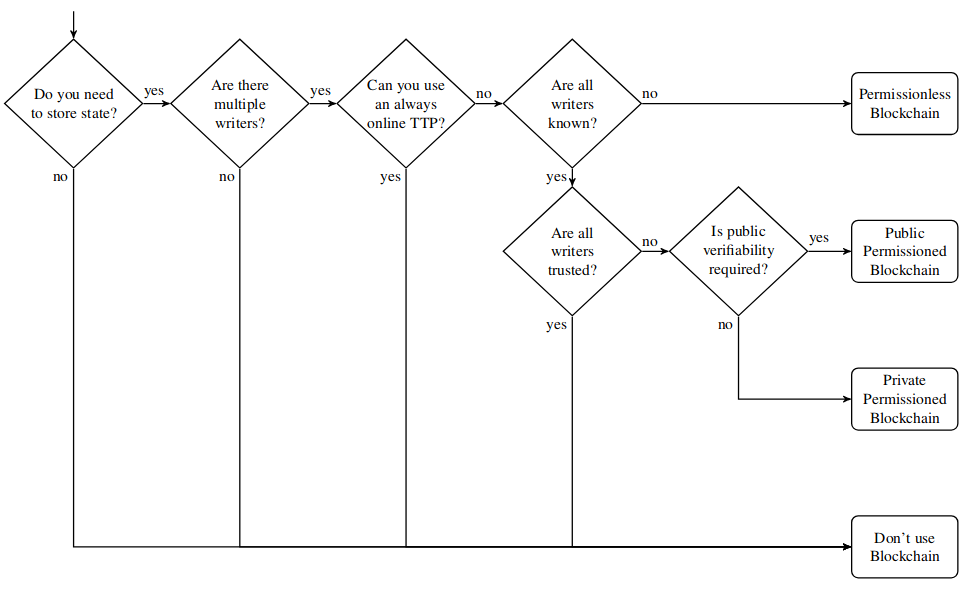
\includegraphics[width=1.0\textwidth]{blockchain_need}
    \caption["Do you need a blockchain?" flowchart]
        {"Do you need a blockchain?" flowchart \citep[p.3]{wust2017you}}
    \label{fig:blockchain_need}
\end{figure}

\citet[p.3]{wust2017you} proposed a decision flowchart (figure \ref{fig:blockchain_need}) to determine whether a blockchain is 
the appropriate solution for a problem, and which type of blockchain is the most appropriate. We could analyse our problem at 
hand using these steps:

\begin{enumerate}
    \item \textbf{Do you need a store state?} Yes. Records in an e-learning system require secure storage.
    \item \textbf{Are there multiple writers?} Yes. There are many different authorities, institutions, educators and learners 
    involved in an e-learning blockchain that demands write assess into records.
    \item \textbf{Can you use an always online Trusted Third Party (TTP)?} \citet[p.2]{wust2017you} described two options of 
    using a TTP: delegate write operations completely to the TTP if it is always online so that it verifies all state 
    transitions, or use the TTP as a certificate authority in the setting of a permissioned blockchain if the TTP is usually 
    offline.\\ 
    In the e-learning context, a TTP could be the e-learning platform provider. However, the delegation of write operations 
    to the platform goes against modern principles of autonomy and independence for higher education institutions. 
    Governmental education ministries in most modern states audits and regulates higher education without writing student 
    records or conferring degrees. An always online TTP should not be used in order to replicate the real world context. This 
    project will answer no for this step.
    \item \textbf{Are all writers known?} Yes. Users of the system should be registered and not be anonymous to the system 
    administrators. [TODO: Why? Are there arguments to anonymous education?]
    \item \textbf{Are all writers trusted?} No. Malpractices from education institutions can occur, especially in the private, 
    for-profit sector. In a future open e-learning market, it could also be possible for anyone to start offering education 
    services. We cannot assume that all writers are trusted.
    \item \textbf{Is public verifiability required?} Yes. One of the objectives of this project is to boost trust in e-learning 
    credentials by increasing public verifiability of education journeys, increasing public accountability especially for 
    stakeholders such as employers and postgraduate studies providers.
\end{enumerate}

This process led to the recommendation of a \textbf{public permissioned blockchain} for this project.

\subsection{Properties of Smart Contracts}
Again, smart contracts are logic embedded in a blockchain that defines the rules and penalties around an agreement and 
could automatically enforce those obligations \citep{gulhane2017ibm}. The term "chaincode" is also used interchangeably 
as a synonym for smart contracts \citep[p.6]{valenta2017comparison}.

There are three main properties of smart contracts:

\begin{itemize}
    \setlength\itemsep{0.2em}        
    \item \textbf{Autonomous}: after launching and running, no further communication is required between a smart contract 
    and its initiating agent;
    \item \textbf{Self-sufficient}: a smart contract should have the ability to keep itself alive when it needs to be, 
    such as raising funds by providing services, and spending them on computing power or storage;
    \item \textbf{Decentralised}: a smart contract does not exist on a single server, they are distributed and self-executing 
    across all of the blockchain peers.\\ 
    \citet[p.16]{swan2015blockchain} 
\end{itemize}

These properties ensure effective operation of the logic defined. In an e-learning context, this can potentially 
be used to govern how teaching, evaluation and feedback take place, enhancing protection for the consumers/ learners.

\section{Existing Efforts in Blockchain for Education}

% chapter 1
% The potential of blockchain enabled systems in education has been noted by the community, with \citet[p.62]{swan2015blockchain} 
% proposing that “learning smart contracts could automatically confirm the completion of learning modules through standardized 
% online tests”. Appropriate configurations in permissions and visibility can also provide improved security and privacy to e-Learning.

\subsection{Blockcerts}

Blockcerts is an open standard for blockchain certificates led by MIT’s Media Lab. Education providers can use it to store 
the records of certifications they have awarded (See figure \ref{fig:blockcerts}). One bitcoin transaction is performed for 
every batch of certificates, with the certificates stored in the OP\_RETURN transaction field on the bitcoin blockchain. 
This is paid for by the certificate issuer. \citep{blockcerts2018}

\begin{figure}[!h] 
    \centering    
    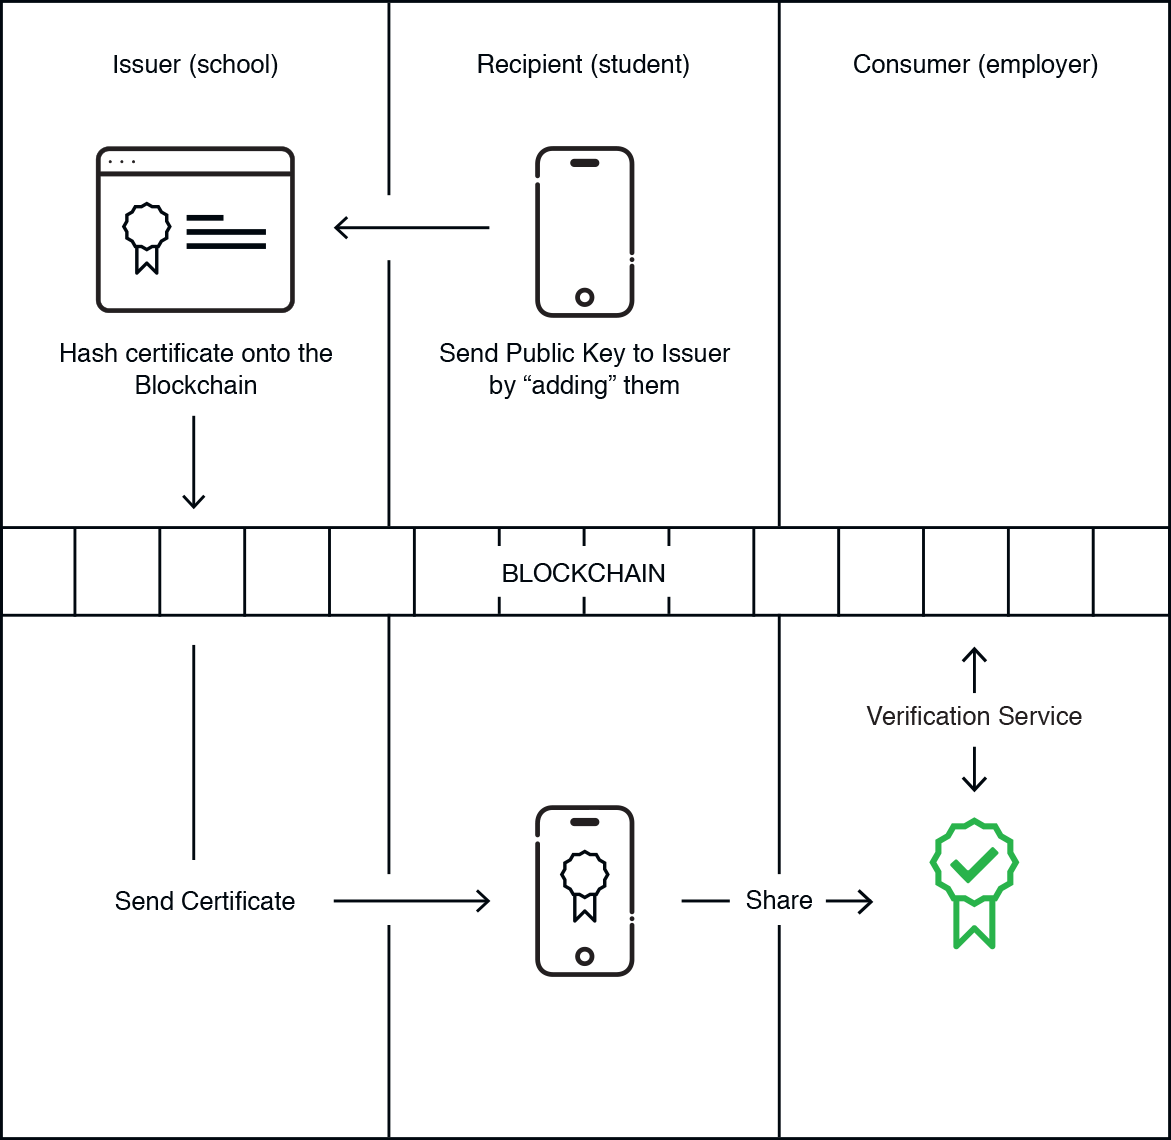
\includegraphics[width=0.7\textwidth]{blockcerts}
    \caption[How Blockcerts work]
        {How Blockcerts work \citep{blockcerts2018}}
    \label{fig:blockcerts}
\end{figure}

\subsection{Sony Global Education Blockchain}% https://blockchain.sonyged.com/

The Sony Global Education Blockchain is based on the Hyperledger project, an open source distributed ledger 
for businesses. It provides an application program interface (API) for developers at education institutes, 
allowing integration with third party applications. It aims to provide tamper-proof, secure storage of 
learning history data for institutions. \citep{sonyged2017}

\begin{figure}[!h] 
    \centering    
    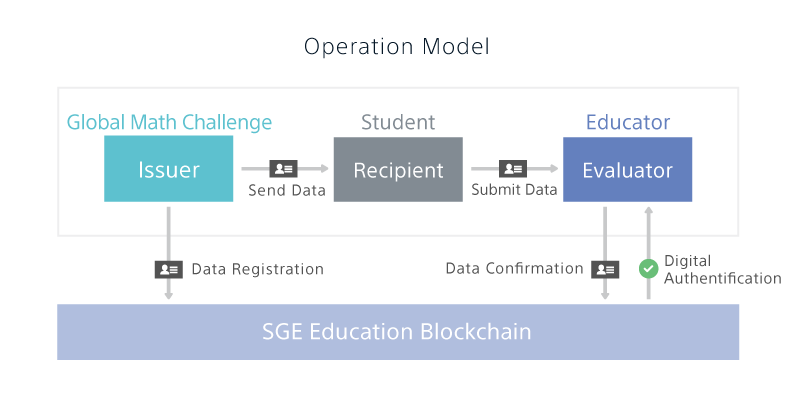
\includegraphics[width=0.7\textwidth]{sonyged}
    \caption[Sony Global Education Blockchain]
        {Operation Example of the Sony Global Education Blockchain \citep{sonyged2017}}
    \label{fig:sonyged}
\end{figure}

\subsection{OpenLearn Blockchain}% http://blockchain.open.ac.uk/

\begin{figure}[!h] 
    \centering    
    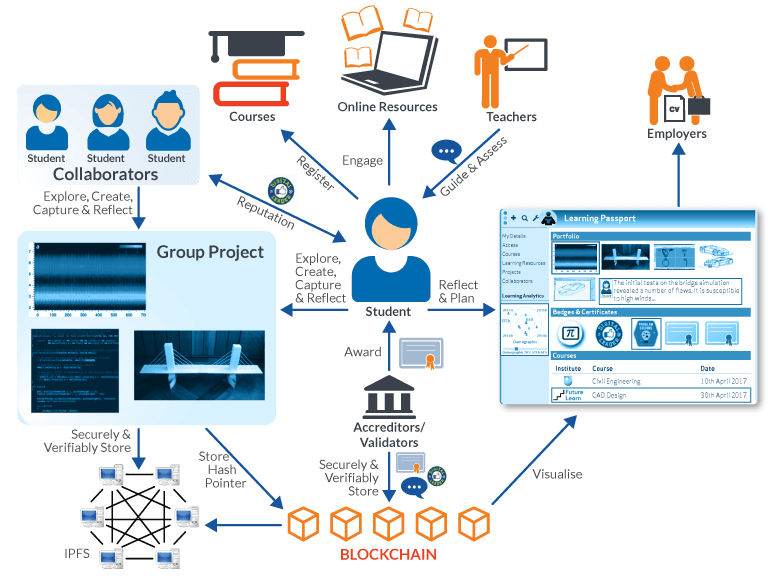
\includegraphics[width=0.95\textwidth]{openlearn}
    \caption[OpenLearn Blockchain scenario]
        {A typical education scenario with the OpenLearn Blockchain\citep{openlearn2018}}
    \label{fig:openlearn}
\end{figure}

The OpenLearn Blockchain project envisions the creation of blockchain based ePortfolios (See figure 
\ref{fig:openlearn}). They are currently demonstrating this with an experimental plugin for Moodle, 
a popular course management system, with which achievement badges can be stored on the Ethereum 
blockchain. This system currently allows students to register for courses and receive badges which 
can be viewed in a student Learning Passport. The transactions are peer-to-peer: in principle no 
host institution is required for the awarding of accreditation. \citep{sharples2016blockchain}

\subsection{Novelty of the proposed project}

\begin{figure}[!h] 
    \centering    
    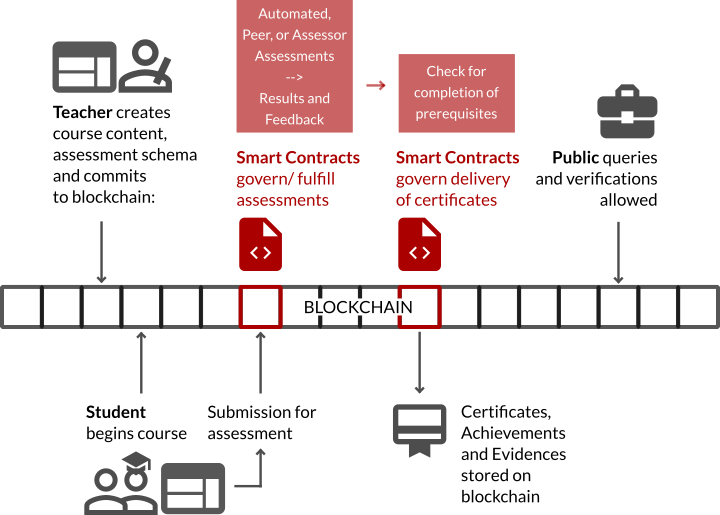
\includegraphics[width=0.95\textwidth]{moocon}
    \caption[Assessment Smart Contracts Concept]
        {Original diagram providing a high level view of how the project proposes automating assessments 
        with smart contracts}
    \label{fig:moocon_assess}
\end{figure}

All of the above three notable efforts focus on identity management and record keeping for education. 
This project will aim to extend these efforts by proposing smart contracts that automate assessments 
(See figure \ref{fig:moocon_assess}) and deliver personalised curricula. 

The vision of this project will also be to create an e-Learning marketplace that teachers can use directly, 
instead of a blockchain network that education providers will have to consume through APIs. This makes for a 
lower cost of entrance in terms of technological know-how and investment.

\section{Overview of Blockchain Development Toolkits}

This project will involve the design of smart contracts for e-Learning transactions and building a demonstrator 
network and applications. A review of the popular blockchain implementations and development toolkits on the 
market is necessary. See table \ref{table:blockchainscomparison} for a overview and below for more commentary.

\begin{table}[!hb] 
    \caption{Comparison of key blockchain implementations, adapted from \citet{ibm2018hyperledger} and \citet{valenta2017comparison}}
    \centering
    \label{table:blockchainscomparison}
    \begin{tabular}{l c c c c}
        \toprule
        & Bitcoin & Ethereum & Hyperledger Fabric & R3 Corda\\ 
        \midrule
        Governance & developers & developers & Linux Foundation & R3 \\\hline
        Crypto- & bitcoin & ether, user-created & none, user-created & none \\ 
        currency & & cryptocurrencies & cryptocurrencies\\\hline
        Network & permissionless, & permissionless, & permissioned, & permissioned,\\ 
        & public & public or private & private & private\\\hline
        Transactions & anonymous & anonymous or & public or & \\ 
        & & private & confidential \\\hline
        Consensus & proof of work & proof of work & PBFT & PBFT\\ \hline
        Smart & none & yes (Solidity, & yes (chaincode) & yes (chaincode)\\ 
        Contracts & & Serpent, LLL) \\\hline
        Language & C++ & Golang, C++, & Golang, Java, & Kotlin, Java,\\
        & & Python & JavaScript & legal prose\\
        \bottomrule
    \end{tabular}
\end{table}

Bitcoin is included in the table only as a point of reference, building with the bitcoin 
blockchain is not considered for this project because of its lack of support for smart 
contracts (any kind of embedded logic or programmes).

\subsection*{Ethereum}

Ethereum is famous for its Turing-complete smart contracts capabilities, which allows entire 
decentralised applications (dApps) to run autonomously on its blockchain. It has a build-in cryptocurrency 
"Ether", which is used to reward miners that contribute to consensus, and to pay transaction fees. 
Developers of dApps can also issue their own currency inside their smart contracts.

\citet[p.3-4]{valenta2017comparison} noted that compared with Ethereum, which makes records accessible 
to all participants, permissioned blockchains such as Fabric and Corda provide "more fine-grained access 
control to records and thus enhance privacy". 
They also achieves higher performance due to a faster consensus mechanism that does not involve mining.

For this project, another crucial consideration against the adoption of the Ethereum environment is the 
lack of a central authority, which makes it impossible for the platform to kick unscrupulous actors off 
the blockchain.

\subsection*{Hyperledger Fabric}

\citet[p.7]{valenta2017comparison} described Fabric as a highly flexible "versatile toolbox". It 
has different roles for peers within the network, where they can act as clients (end users), peers 
(record keepers), endorsers (transaction verifiers), or orderers (transaction requester). The 
consensus mechanism is by default a Byzantine fault-tolerant (BFT) algorithm and can be customised. 
A cryptocurrency is not required, but could be developed with chaincode.

\subsection*{R3 Corda}

Built following use cases in the financial industry, Corda notably augmented smart contracts 
with legal prose, making it a great tool for highly regulated environment. The development of 
a cryptocurrency is not intended or supported. \citep{valenta2017comparison}

Education is not a highly regulated environment and this unique selling point of Corda is not 
immediately attractive to this project.

\subsection*{Summary}

Combining the recommendation for a public permissioned blockchain from the framework provided 
by \citet{wust2017you} (See Section 2.1.1), and the brief analysis above, Hyperledger Fabric 
stands out as the best platform which could allow for a lot of future work. Backed by the 
Linux Foundation, Hyperledger projects have extensive documentations and a large, 
active community. 

The discussion following this chapter will now commit to using Hyperledger 
Fabric as the blockchain platform for this project.

% http://explore-ip.com/2017_Comparison-of-Ethereum-Hyperledger-Corda.pdf